Scaling up a DDMS requires not only storing progressively more data, but also a
dramatic increase in computing resources.  As alluded to in Section
\ref{sec:storage}, DDMS and their corresponding transition programs are amenable
to having their data distributed across a cluster: (1) The only data structures
used by transition programs are maps, which are amenable to horizontal
partitioning.  (2) At the granularity of a single update, iterative computations
are completely data-parallel. 
\comment{(3) \note{The effect of a sequence of updates
(i.e., executing the corresponding trigger functions) is independent of the
order in which the updates are applied.}}

\tinysection{Update Processing Consistency and Isolation}
\comment{
\note{Though order of execution is irrelevant at the granularity of
updates,}}
In DBToaster, transition functions are created under the assumption that they
are operating on a \textit{consistent} snapshot of the DDMS's state. The entire
sequence of statements composing the trigger function must be executed
atomically, to ensure that each statement operates on maps resulting from fully
processing the update stream prior to the update that fired the trigger.
Thus the effects of updates should be fully isolated from each other.
Similar issues and requirements have been raised before in the single-site
context of view maintenance with the ``state bug''~\cite{colby-sigmod:96}.

Our requirement of processing updates in such an order is conservative, indeed
we could apply standard serializable order concurrency control here to
simultaneously process updates that do not interact with each other. The
underlying goal is to develop simple techniques that avoid heavyweight locking
and synchronization of entries in massively horizontally partitioned maps. 
We start with a conservative goal to focus on simple lightweight protocols.
Ensuring this atomicity property is the first of the two core challenges that we
encountered while constructing a distributed DDMS runtime.

\tinysection{Distributed Execution}
Each update in our distributed DDMS runtime design employs three classes of actor:
\begin{itemize}
\item \textit{source nodes}: Nodes hosting maps read by the update's trigger
function (maps appearing on the right-hand side of the function's statements).
\item \textit{computation nodes}: The nodes where statements are evaluated.
\item \textit{destination nodes}: Nodes hosting maps written to by the update's
trigger function (maps appearing on the left-hand side of the function's
statements).
\end{itemize}
Note that these actors are logical entities; it is not necessary (and in fact,
typically detrimental) for the actors to be on separate physical nodes within
the cluster.
\comment{
\note{Unfortunately, distribution always introduces some amount of
separation; the source nodes for one update will be the destination nodes for
another, and visa versa.}
}
Introducing a distinction between the different tasks involved in
update processing allows us to better understand the tradeoffs involved in the
second core challenge: selecting an effective partitioning scheme that
intelligently determines placements of logical entities in order to best
utilize plentiful hardware to handle a large update stream and DDMS state.

\subsection{Execution Models}
We first address the issue of atomicity by providing two execution models: (1) A
protocol that provides a serial execution environment for transition programs,
and (2) An eventual consistency protocol that provides the illusion of serial
execution.

\tinysection{Serial Execution}
The most straightforward way of achieving atomicity is to ensure serial trigger
function execution.  However, requiring all nodes in the cluster to block on a
barrier after every update is not a scalable approach. A similar effect can be
achieved more efficiently by using fine-grained barriers, where each update is
processed by first notifying all of the update's destination nodes of an
impending write. Reads at the update's source nodes are blocked while writes
from prior updates are pending.

Serial execution requires a global ordering of updates as they arrive at
the DDMS. Techniques to achieve this include:
\begin{itemize}
\item Updates arrive only from a single producer (e.g., the cluster is
maintaining a data warehouse that mirrors a single OLTP database).
\item A central coordinator generates a global ordering (as in
\cite{peng-incremental:10}).
\item A distributed consensus protocol generates a global ordering (as in
\cite{Junqueira:2009:LTZ:1582716.1582721}).
\item A deterministic scheme produces a global ordering. For example, each
update producer generates timestamps locally and identical timestamps in a
global view are settled with a deterministic tiebreaker like the producer's IP
address.
\end{itemize}

We also need a mechanism to provide consistent delivery of updates from multiple
producers. Before completing a read, source nodes must not only ensure that all
prior pending writes have been completed, but also that all notifications for
prior updates have been received.
A simple solution is to channel all updates through a single server. This has
the advantage of also providing a global ordering over all updates.  However
this solution creates a scalability bottleneck.  Alternative solutions like
broadcasting updates or periodic commits are possible, but introduce
considerable synchronization overheads.

\tinysection{Speculative Execution with Deltas}
As an alternative, we can favor the use of speculative and optimistic processing
techniques in designing our distributed execution protocol. The key insight here
is that our computation is based on incremental processing, thereby unlike
standard usage of speculative execution, any work done speculatively need not be
thrown away entirely, rather any work done can be revised through increments or
deltas, to the final desired outcome.

In particular, a node can optimistically perform reads immediately without
blocking (or at least, blocking only on pending write operations which the node
is already aware of, and not the vague possibility of potential future write
operations).  Although avoiding blocking on potential future writes eliminates
significant synchronization overheads, out-of-order updates can cause the
atomicity and desired ordering properties of trigger execution to be lost.
\comment{
\todo{it negates the assumption of atomicity that transition programs are
constructed with}.}
We favor this point in the design space since out-of-order events are expected
to occur infrequently. Furthermore, such events are likely to interfere with
only a handful of prior updates, for example a write on one map entry followed
by an out-of-order read on a different entry in the same map do not cause a
problem. Finally, because write operations are limited to additive deltas,
there is a clear mechanism for composing out-of-order write operations.

\comment{
\todo{We begin to restore the assumption of atomicity} by using a timestamping
mechanism (one of the several options described above) to establish a ``correct"
order of operations between the updates.  However, without synchronization
measures, it is possible for updates to arrive out of order.  Frequently, this
will not be an issue -- a write on one map entry followed by an out-of-order
read on a different entry in the same map do not cause a problem.  Furthermore,
because write operations are limited to additive deltas, there is a clear
mechanism for composing out-of-order write operations.
}

\begin{figure}
\begin{center}
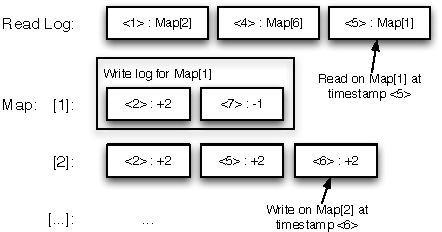
\includegraphics[width=3.0in]{graphics/speculative_storage}
\end{center}
\caption{Supplemental data structures used to facilitate speculative execution in a distributed DDMS.}
\label{fig:speculativeStorage}
\vspace{-3mm}
\end{figure}

\tinysection{Out-of-Order Processing with Deltas as Revisions}
\comment{
Error correction in the speculative execution model requires the ability to
}
We handle two types of out-of-order operations: write-before-read, and
read-before-write.  We supplement maps with two additional data structures
capturing timestamp information for operations, as illustrated in Figure
\ref{fig:speculativeStorage}: (1) Source nodes maintain a log of all read
operations.  (2) Destination nodes save all write operations independently; map
entries are saved as logs rather than summed values.  Each operation is tagged
with and sorted by the effecting update's timestamp \texttt{<t>}.

%\tinysection{Out-of-order Reads}
In the case of an out-of-order read operation (i.e., one that arrives after a
write operation that logically precedes it), the write log makes it possible to
reconstruct the state of the map at an earlier point in time.
For example, given the initial state in Figure \ref{fig:speculativeStorage}, an
update that requires a read on entry \texttt{Map[2]} arrives with timestamp
\texttt{<3>}.  The value sent to the computation nodes is not the latest value
of the entry ({\tt Map[2]} $ = 6$ for all timestamps after {\tt <6>}), but
rather the sum of all values with lower timestamps ({\tt Map[2]} $ = 2$ for
timestamps {\tt <3>},{\tt <4>}, and {\tt <5>}).

%\tinysection{Out-of-order Writes}
In the case of an out-of-order write operation, the read log allows us to send a
\textit{revising update} to each computation node affected by the write.
For example, given the initial state in Figure \ref{fig:speculativeStorage}, an
update that requires a write on entry \texttt{Map[6]} arrives with timestamp
\texttt{<3>}.  The value will be written as normal (i.e., inserted into the
write log for \texttt{Map[6]}, in sorted timestamp order).  Additionally,
because the read log shows a read on the same entry with a later timestamp, a
corrective update will be sent to the computation node(s) to which the entries
were originally sent to.

%\tinysection{Bounding Memory Usage}
Both data structures grow over time.  To prevent unbounded memory usage,
it is necessary to periodically truncate, or garbage collect the entries in each. 
This in turn, requires the runtime to periodically identify a cutoff point; the
``last" update for which there are no operations pending within the cluster. 
The read history is truncated at this point, and all writes before this point
are coalesced into a single entry.  Though this process is slow, it does not
interfere with any node's normal operations, and can be performed infrequently;
once every few seconds is reasonable.

\tinysection{Hybrid Consistency}
\comment{
\todo{A potential drawback of the speculative execution model is that it
produces eventual consistent results}; unless the system quiesces, there is no
guarantee that the sum of all entries in the write history of the result map
will be representative of the actual query results at some point in the update
stream.}
While the speculative execution model and its eventually consistent results are
advantageous from a performance and scalability perspective, there may not be a
point at which the state of all maps in the system corresponds to a consistent
snapshot of our transition programs evaluated over any prefix of the update
stream.
That is, there is no guarantee that the system has actually converged to its
eventually consistent state in the presence of a highly dynamic update stream.
However, a side effect of the garbage collection process is that each garbage
collection run, in effect generates a consistent snapshot of the system. As in
other eventual consistency systems~\cite{bayou}, this approach offers a hybrid
consistency model, specifically the same infrastructure produces both
low-latency eventually consistent results, as well as higher-latency consistent
snapshots.

\subsection{Partitioning Schemes}
The second challenge associated with distributing a transition program across
the cluster is the distribution of logical nodes (source, computation, and
destination) across physical hardware in the cluster.  In addition to more
complex, min-cut based partitioning schemes for the data, DBToaster considers
two simple partitioning heuristics for distributing computation:
(1) data shipping: evaluate program statements where their
results will be stored, at destination nodes, or
(2) program shipping: evaluate program statements where their input maps are
stored, at source nodes.

\tinysection{Destination-Computation}
Given the one-to-one correspondence between computation nodes and destination
nodes, the simplest partitioning scheme is to perform computations where the
data will be stored -- that is, the destination and computation nodes are
co-located.  As part of update evaluation, each source node transmits all
relevant map entries to the destination node.  Upon arrival, the destination
node evaluates the statement and stores the relevant results.

\tinysection{Source-Computation}
Though simple, transmitting every relevant map entry with every update can be
wasteful, especially if the input map entries don't change frequently.  An
alternative approach is to co-locate all of the source nodes and the computation
node.  When evaluating an update, the computation can be performed
instantaneously, and the only overhead is transmitting the result(s) to the
destination node(s).  This is particularly effective in queries where update
effects are small (e.g., queries consisting mostly of equijoins on key columns).

However, this approach introduces an additional complication.  It is typically
not possible to generate a partitioning of the data that ensures that for each
statement in a trigger program, all the source nodes will be co-located.  In
order to achieve a partitioning, data must be replicated; each map is stored on
multiple physical nodes.  While replication is typically a desirable
characteristic, storage-constrained infrastructures may need to use
complex partitioning schemes.

